
\pdfminorversion=4





\documentclass[11pt]{article}
\usepackage{amsmath, amsthm}
\usepackage[pdftex]{graphicx}
\usepackage{psfrag,epsf}
\usepackage{enumerate}
\usepackage{natbib}
\usepackage{float}
\restylefloat{table}

\usepackage{amssymb}
\usepackage{multirow}
\usepackage{float}
\newtheorem{thm}{Theorem}

\newcommand{\blind}{0}

\addtolength{\oddsidemargin}{-.75in}%
\addtolength{\evensidemargin}{-.75in}%
\addtolength{\textwidth}{1.5in}%
\addtolength{\textheight}{1.3in}%
\addtolength{\topmargin}{-.8in}%

\newtheorem{theorem}{\bf Theorem}
\newtheorem{proposition}{\bf Proposition}
\newtheorem{lemma}{\bf Lemma}
\newtheorem{corollary}{\bf Corollary}
\numberwithin{equation}{section}

\date{\textbf{Draft} \textbf{\today}}
\begin{document}

%\bibliographystyle{natbib}

%\newcommand{\keywords}[1]{\par\addvspace\baselineskip
%\noindent\keywordname\enspace\ignorespaces#1}

\def\spacingset#1{\renewcommand{\baselinestretch}%
{#1}\small\normalsize} \spacingset{1}


%%%%%%%%%%%%%%%%%%%%%%%%%%%%%%%%%%%%%%%%%%%%%%%%%%%%%%%%%%%%%%%%%%%%%%%%%%%%%%

\if0\blind
{
  \title{A Shape Constraint with Heavier Tails: Inverse Convex}
  \author{Clifford Anderson-Bergman\\
    Department of Statistics, University of California Berkeley\\
    }
  \maketitle
} \fi

\if1\blind
{
  \bigskip
  \bigskip
  \bigskip
  \begin{center}
    {\large\bf A Shape Constraint with Heavier Tails: Inverse Convex}
\end{center}
  \medskip
} \fi


\spacingset{1.4}


\begin{abstract}

	The shape constraint of log concavity is considered a fairly flexible constraint, as many classic parametric families are contained within the family, it allows for skew and up to exponential tails. However, in certain situations this may still not be considered heavy tailed enough, such as survival analysis or modeling income. To address this, we present a new shape constraint: inverse convex. We show that the family of log-concave distributions is completely contained within the family of inverse convex, present several classic parametric families which are not log-concave but are inverse convex and examine other interesting characteristics of the inverse convex constraint, including the heavy tails. Although the likelihood is unbounded, we provide an algorithm which finds a finite local maximum of the likelihood function reliably for moderate samples ($n > 25$) and show that this estimator has favorable characteristics when modeling heavy tailed data. We use our new estimator and two other comparable estimators on two income dataset, one collected by the Philippines' National Statistics Office and one collected by the US Census. 
	
\end{abstract}

 {\bf Keywords}: Non-parametric, Shape Constraints, Log-Concave, Inverse Convex

{\section{A New Shape Constraint: Inverse Convex} } 

	Shape constrained non-parametric maximum likelihood estimation of density functions involves making a robust assumption of the shape of the target distribution and maximizing the likelihood such that the estimated density function respects the shape constraint. Recent applications of such shape constraints include univariate density estimates (Rufibach 2007), survival estimation (Anderson-Bergman and Yu 2014) or as part of a more complex model, such as components of a mixture model (Chang and Walther 2007) and as a baseline distribution for a Cox PH model (Anderson-Bergman 2014). The motivation for use of  shape constrained estimation is one can greatly improve the operating characteristics of a non-parametric estimator by enforcing mild constraints, while not requiring the investigator limit the density function to a fully parametric family or select an uninterpretable smoothing parameter. In some cases, the shape constraint is necessary for inference. For example, the empirical distribution function leads to degenerate density estimates, but simple shape constraints can lead to consistent density estimation (Grenander 1956, Rufibach 2007). In other cases, the variance of non-parametric estimates is greatly reduced by using shape constraints. For example, survival estimates using the unconstrained NPMLE for interval censored data are notoriously inefficient (Groeneboom 1991), but applying shape constraints can improve this considerably (Anderson-Bergman and Yu  2014). 
			
	The earliest shape constraint to appear in the literature was the decreasing density constraint, also known as the Grenander estimator (Grenander 1956). After the Grenander estimator, a tempting constraint considered was that of uni-modality. However, this estimator is degenerate if the mode is not known in advance, as the estimator will place infinite density at the mode (Wegman 1969). A shape constraint that has received considerable amount of attention recently is the log-concave constraint (D\"umbgen and Rufibach 2009, Chang and Walther 2007, D\"umbgen \emph{et al} 2011, Anderson-Bergman 2014, Anderson-Bergman and Yu 2014). The constraint of log-concave implies $f_X(x) = \exp ( {\phi(x)} )$, where $\phi(x)$ is a concave function. This constrained estimator has the properties of being uni-modal, allowing for skew and providing consistent density estimates. 
	 
	 In certain situations, the log-concave constraint may not allow for heavy enough tails. In survival analysis, the exponential distribution is often considered a standard model. The exponential distribution is on the boundary of log-concave (log linear), so the constraint of log concavity cannot be considered robust to heavy tails in survival analysis. Viewing the same problem from another angle, the constraint of log concavity insures an increasing hazard function, so will be inadequate for modeling distributions which may have decreasing hazards. 	
	 
	 To address these concerns in survival analysis and other types of heavy tailed data, we introduce a new, more flexible shape constraint. We will call this constraint ``inverse convex". In section 2, we examine some interesting characteristics of the family of inverse convex distributions, including proving that the log-concave family is a proper subset of the inverse convex family, with inverse convex allowing for heavier tails. In section 3, we discuss characteristics of the likelihood function. Of particular interest is the fact that the likelihood function is unbounded, but a local finite mode provides satisfactory estimates, similar to a Gaussian mixture problem without fixed variance components. In section 4, we briefly introduce the algorithm used to find the inverse convex estimator, although we skip the details as it is a simplified version of the algorithm presented in Anderson-Bergman and Yu 2014 (can also be found in Anderson-Bergman 2014). We also demonstrate that our algorithm can reliably find the local mode of interest for reasonable sample sizes ($n > 25$) and that our algorithm converges to the same mode, regardless of initial values of the algorithm. In section 5, we present simulation results to examine the performance of the inverse convex estimator as compared to the log concave estimator. In section 6, we apply the inverse convex to real data. In section 7, we discuss the findings of this study.
	 
	 While we believe this estimator is very attractive for survival analysis for censored data, the algorithm we have implemented does not allow for censoring yet. Based on our work with the log-concave estimator, we believe such an algorithm should not require novel optimization methods beyond what we have already done. However, it will take some time to implement these tools. 
	 
	 
{\section{Characteristics of the Inverse Convex Family} }
		
	We start by defining the inverse convex family. We say that $f(x)$ is inverse convex if $f(x) = 1/g(x)$ such that $g(x)$ is a convex function. We will call $g(x)$ the inverse kernel.  Much like the log-concave constraint, the inverse convex constraint implies a distribution to have no more than one peak (although both can be flat like a uniform distribution), as $g(x)$ can only have one locally minimum region. An attractive feature of the inverse convex family is that the log-concave family is a subset. To show this, consider that $f(x)$ is log-concave if $f(x) = e^{\phi(x)}$ such that $\phi(x)$ is concave. If we can show that $e^{-\phi(x)}$ is convex, we have shown log-concave implies inverse convex. Because $\phi(x)$ is concave, $-\phi(x)$ is convex, making $e^{-\phi(x)}$ log convex. Log convex implies convex, therefore $e^{-\phi(x)}$ is a convex function.  Thus, log-concave implies inverse convex. 
	
		
	In addition, several classic parametric distributions which are not log-concave are still inverse convex. For example, any t-distribution, the F-distribution with $\nu_1$ (or $df_1$) $\geq 2$ and  log logistic distribution with $\beta \geq 1$ are inverse convex distributions but are not log-concave. 

	Several classic distributions are excluded from the family of inverse convex distributions. Any multimodal distribution cannot be inverse convex. In addition, any non-degenerate distribution with unbounded density, such as the F-distribution with $\nu_1 < 2$ or the log logistic with $\beta < 1$, cannot be an inverse convex distribution. We will use a proof by contradiction to show this. 
	
	Suppose $f(x)$ is a non-degenerate inverse convex distribution, such that $\displaystyle \lim_{x \rightarrow x_0} f(x) = \infty$ (or $\displaystyle \lim_{x \rightarrow x_0} g(x) = 0$) from at least one side . Because $f(x)$ is non degenerate, there must exist $\delta$ with $| \delta | > 0$ such that $f(x_0 + \delta) = a > 0$. For notational simplicity, we will assume $\delta > 0$, although this proof trivially generalizes to $\delta < 0$ as well. We can bound $\displaystyle \int_{x_0}^{x_0 + \delta} f(x) \mathrm{d}x$ from below with a function which is inverse linear between $x_0$ and $x_0 +\delta$, as this is the boundary of an inverse convex distribution. Applying this bound, 
	
	\[
	f(x) \geq \left( g(x_0) + (x - x_0) \frac{g(x_0 + \delta) - g(x_0) } {x_0 + \delta - x_0} \right)^{-1} \text{ , } x \in (x_0, x_0 + \delta)
	\]
	
	Plugging in $g(x_0) = 0$, $g(x_0 + \delta) = a^{-1}$ and simplifying, we get 
		
	\[
	f(x) \geq \frac{a \delta}{x - x_0}  \text{ , } x \in (x_0, x_0 + \delta)
	\]	
		
	Integration leads to 	
		\[
		\displaystyle \int_{x_0}^{x_0 + \delta} f(x) \mathrm{d}x \geq  \displaystyle \int_{x_0}^{x_0 + \delta} \frac{a \delta}{x - x_0} \mathrm{d}x
		 = a \delta \displaystyle  \int_0^{\delta} \frac{1} {x} \mathrm{d}x = \infty
		\]
		
	This leads to an improper distribution. Therefore, there are no proper inverse convex probability functions with unbounded density. Interestingly, the lognormal distribution with $\sigma > 2$ is not inverse convex, despite having bounded density. Particularly, the distribution is non-inverse convex on the interval $(e^{\mu - \sigma^2/2 - \sqrt{\sigma^4 - 4\sigma^2} } , e^{\mu - \sigma^2/2 + \sqrt{\sigma^4 - 4\sigma^2}} )$, where the density becomes extraordinarily peaked. In contrast, the log normal is not log-concave for all values of $\sigma > 0$. 
	
	We emphasize that the key difference between the log-concave constraint and the inverse convex constraint concerns the heavy tails. The boundary of the log-concave constraint is an exponential tail, which may be insufficient in some cases. The boundary of the tails of an inverse convex distribution, as defined by the shape constraint alone, is an inverse linear function. However, because a positive inverse linear function will integrate to $\infty$ over $[a, \infty)$ for any $a$, in order for an inverse convex distribution to be a proper distribution function, the tails must not be on the boundary of the inverse convex constraint. This implies that the inverse convex constraint will not limit the weight of the tails of a distribution. 
	
		This feature of heavy tails can be especially attractive for survival analysis with heavy censoring. For example, consider if investigators are conducting a study in which the study began at time $t = 0$ and ends at $t = 1$, so any events occurring after $t = 1$ are right censored. Suppose we found that the fit $\hat f_X(x) = 0.5 e^{-x}$ describes the data quite well over $t = [0,1]$. Although this function is log-concave over [0,1], we cannot fit a log-concave estimator to have this fit over [0,1], as it is not possible to assign enough probability mass over $[1, \infty)$ so that our estimate would be log-concave and a proper distribution function. This is because the mass assigned would be maximized by extending the function over $[1, \infty)$, leading to $\hat f_X(x) = 0.5 e^{-x}$, $0 < x < \infty$, which integrates to 0.5. This has the unpleasant result that we cannot fit the data well because of the behavior over the area we have not observed, despite being a good fit over the area we have observed. On the other hand, if we used an inverse convex estimator and the fit appeared good over $t = [0,1]$, then we will always be able to assign enough mass over $[1, \infty)$ to form a proper distribution function, as the amount of mass we can assign is unbounded. Thus, we only need to worry about the fit over the observed area rather than the fit over both the observed and censored data. 

			
{\section{Characterization of the Inverse Convex Estimator} } 

	A displeasing characteristic of the inverse convex estimator is that the log likelihood function is unbounded, as we will show in this section. In particular, as the estimate approaches a degenerate distribution about a single observed value, the likelihood approaches infinity. However, in practice, we find that the algorithm we present in section 4 typically convergences to a non-degenerative, informative estimate. This is very similar to the case of the Gaussian mixture model, in which the likelihood function is unbounded, but estimates which are local modes with finite likelihood lead to valid estimation. Empirically, we find our algorithm converges to a unique finite mode with very high probability for all but the smallest of samples, as will be demonstrated in section 4. 
	
	{\subsection{Parameterization of the Likelihood Function} } 
	
	The likelihood function can be written in the form
	
	\[
	\ell(g| x ) =  \displaystyle \sum_{i = 1}^n -\log(g(x_i))
	\]
	
	\[
	\text{with constraints } \frac{g(x_2) - g(x_1)} { x_2 - x_1} \leq \frac{g(x_3) - g(x_2)} { x_3 - x_2} \text{ } \forall x_1 < x_2 < x_3
	\]
	
	\[
	\text{and } \displaystyle \int_{-\infty}^{\infty} g(x)^{-1} \mathrm{d}x = 1
	\]
	
	To ease the last constraint, we will replace $g(x_i)^{-1}$ with $g(x_i)^{-1}/ \displaystyle \int_{-\infty}^{\infty} g(x)^{-1} \mathrm{d}x$. This means that $g(x_i)^{-1}$ is proportional to the estimated density at $x_i$ up to a multiplicative constant. Now we can rewrite the likelihood function as 

	\[
	\ell(g| x ) = \displaystyle \sum_{i = 1}^n -\log(g(x_i)) - n \log\left(\displaystyle \int_{-\infty}^{\infty} g(x)^{-1} \mathrm{d}x \right)
	\]
	
	\[
	\text{with constraints } \frac{g(x_2) - g(x_1)} { x_2 - x_1} \leq \frac{g(x_3) - g(x_2)} { x_3 - x_2} \text{ } \forall x_1 < x_2 < x_3
	\]

	Similar to the log-concave estimator, the inverse convex estimator can  will be described by an inverse linear function with knots at the observed times, as this is a necessary condition for our estimate $\hat g(x)$ to be a local max. We will use an identical argument to the argument  presented in Rufibach (2007) for the log-concave estimator. Let us assume the $x_i$'s are ordered, so that $x_1 \leq x_2 \leq ... \leq x_n$. For any set of values $g(x_1), ... ,g(x_n)$, the likelihood function is maximized by minimizing $\displaystyle \int_{-\infty}^{\infty} g(x)^{-1} \mathrm{d}x$. That means zero mass will be placed below $x_1$ and above $x_n$. In addition, for a given $g(x_i)$, $g(x_{i+1}) $, we maximize the likelihood function by minimizing $\displaystyle \int_{x_i}^{x_{i+1} } g(x)^{-1} \mathrm{d} x $. Because of the constraint of convexity of $g(x)$, this is minimized by making $g(x)$ linear between $x_i$ and $x_{i+1}$. Therefore $\hat g$ will be a piecewise linear spline with knots at the observed values $x_i$. We can completely characterize the solution by $\beta_1,...,\beta_n$, where $\beta_i = g(x_i)$. Under this parameterization, the likelihood function can be written as
	
	\[
	 \ell(\beta | x) = \displaystyle \sum_{i = 1}^n -\log(\beta_i) - n \log \left( \displaystyle \sum_{j=1}^{n-1} \frac{ \log (\beta_{j+1}) - \log (\beta_j) }  { \left( \frac{ \beta_{j+1} - \beta{j} } {x_{j+1} - x_j} \right) } \right)
	\]
	\[
	\text{which satisfy } \frac{\beta_{i+1} - \beta{i} } {x_{i+1} - x_{i} } \leq \frac{\beta_{i+2} - \beta_{i+1}} {x_{i+2} - x_{i+1} }; 1 \leq i \leq n - 2
	\]

	\[\beta_i > 0 \text{; } 1 \leq i \leq n \]

	Note that if $\beta_{i+1} = \beta_i$, the $i^{\mathrm{th} } $ term in the summation is undefined. In this case, the integral over $(x_i, x_{i+1})$ is equal to  $\beta_i^{-1} (x_{i+1} - x_i)$. In addition, the term is undefined if there are ties in the data. To account for this, we will redefine $x_i$ = the $i^{\mathrm{th} } $ \emph{unique} time, $\pi_i$ = number of observations at time $x_i$ and $n^*$ is the number of unique times in the dataset. Note that $\sum_{i = 1}^{n^*} \pi_i = n$. Then we can rewrite the inverse convex likelihood as 
	
	\[
	 \ell(\beta | x) = \displaystyle \sum_{i = 1}^{n^*} -\log(\beta_i)\pi_i - n \log \left( \displaystyle \sum_{j=1}^{n^*-1} \frac{ \log (\beta_{j+1}) - \log (\beta_j) }  { \left( \frac{ \beta_{j+1} - \beta{j} } {x_{j+1} - x_j} \right) } \right)
	\]

	Not only does this allow the likelihood function to handle ties in the data, but it also allows for easy implementation into a mixture model, as $\pi_i$ could just as well represent probability weights. 

%\begin{comment}


	{\subsection{Unbounded Nature of the Likelihood Function} } 
	
	\begin{thm}
	\label{thm3}
	The likelihood function for the inverse convex estimator is unbounded.
	\end{thm}
	
	\begin{proof}
	
	In the case that the of only one unique observed value, the proof is trivial. Let us consider at least two unique points. Recall that by representing the inverse kernel as a linear spline as we did above, the likelihood function can be written as 
	\[
	\ell(\beta) = \sum_{i = 1}^{n^*} -\pi_i \log(\beta_i) - n \log \left( \displaystyle \sum_{j=1}^{n^*-1} \frac{ \log (\beta_{j+1}) - \log (\beta_j) }  { \left( \frac{ \beta_{j+1} - \beta{j} } {x_{j+1} - x_j} \right) } \right)
	\]
	
	Now suppose we consider $g(x)$ to be strictly linear on $[x_1, x_n]$ with $g(x_n) = 1$.  This leads to 
	
	\[
	\beta_i = \beta_1 + \frac{1 - \beta_1} {x_n - x_1} \times (x_i - x_1)
	\]
	
	\[
	\sum_{j=1}^{n^*-1} \frac{ \log (\beta_{j+1}) - \log (\beta_j) }  { \left( \frac{ \beta_{j+1} - \beta{j} } {x_{j+1} - x_j} \right) } =
	\frac{  - \log (\beta_1) }  { \left( \frac{ 1 - \beta_{1} } {x_{n^*} - x_1} \right) }
	\]
	
	Plugging these values in, we can rewrite the likelihood function as 
	
	
	\[
	\ell(\beta_1)= -\pi_1 \log(\beta_1)  - \displaystyle \sum_{i = 2}^{n^*}  \pi_i \log \left( \beta_1 + \frac{1 - \beta_1} {x_{n^*} - x_1} \times (x_i - x_1) \right) - n \log \left( \frac{ - \log(\beta_1)}{ \frac {1 - \beta_1} {x_{n^*} - x_1} } \right)
	\]

	Assuming $\beta_1 < 1$, 

	\[
	= -\pi_1 \log(\beta_1)  - \displaystyle \sum_{i = 2}^{n^*} \pi_i \log \left( \beta_1 + \frac{1 - \beta_1} {x_{n^*} - x_1} \times (x_i - x_1) \right)  - n \log \left( - \log(\beta_1) \right) - n\log \left( \frac {1 - \beta_1} {x_{n^*} - x_1} \right)	
	\]
	
	When taking the limit as $\beta_1 \rightarrow 0$, we note that $\displaystyle \sum_{i = 2}^{n^*} \pi_i \log \left( \beta_1 + \frac{1 - \beta_1} {x_{n^*} - x_1} \times (x_i - x_1) \right) $ and $n\log \left( \frac {1 - \beta_1} {x_{n^*} - x_1} \right)$ both approach a constant.  This leaves us with 
	
	\[
	\underset{\beta_1 \rightarrow 0} \lim \ell(\beta_1) = - \pi_1 \log(\beta_1) - n\log( \log(\beta_1)  ) + c
	\]
	\[
	 = - n\log( \beta_1^{(\pi_1/n)} \log(\beta_1)  ) + c
	\]
	
	By L'H\^opital's rule, this approaches $\infty$ as $\beta_1 \rightarrow 0$. As $\beta_1 \rightarrow 0$, the estimated probability density approaches a degenerate distribution centered around $x_1$. 
	
	\end{proof}

	Because of this, the maximum likelihood estimate is undefined. However, we have found that using a local maximum of the likelihood function leads to a very useful estimation tool, similar to the Gaussian mixture problem. In addition, we found that in practice, avoiding the domain of attraction to the degenerate estimate was quite easy, especially as $n$ becomes larger (making this actually much easier than the Gaussian mixture problem). 

	To present heuristic evidence of the shrinking domain of attraction, we present some toy datasets. We parameterize the estimator as was done in the theorem above, and plot the log likelihood as a function of the single parameter $\beta_1$. In these datasets, the observed values are set to the $\frac{1}{n+1}, ... ,\frac{n}{n+1}$ quantiles of either a uniform(0,1) distribution or an $F_{1,1}$ distribution. We chose a uniform(0,1) for simplicity, as we the mode we are interested in will be known to be $\beta_1 = 1$. We chose an $F_{1,1}$ because this is a distribution which has unbounded density as $x \rightarrow 0$, so we expect the domain of attraction to the degenerate mode to be close to the local mode of interest and we were concerned the domain of attraction to the local mode may blend into the domain for the degenerate mode. The plots for $n$ = 2, 5, and 25 can been seen on figure 1.
	
	\begin{figure}[H]
	\centerline{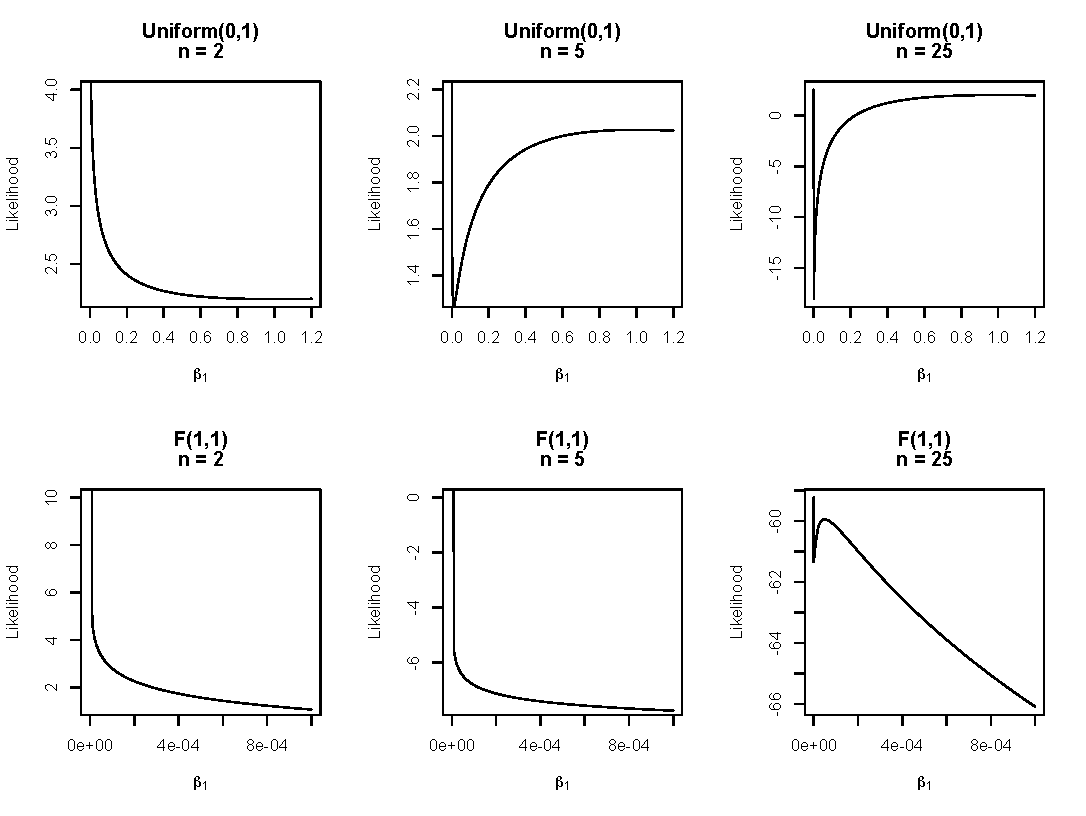
\includegraphics[width = 15cm]{DomainA.pdf} }
	\caption{Likelihood as a function of $\beta_1$}
	\end{figure} 
	
	We note a few things from these plots. First is that for both the uniform and $F_{1,1}$ distribution, the domain of attraction to the degenerate mode appears to be $(0, \infty)$ for the case of $n= 2$. However, for the uniform data points, by $n = 5$, the domain of attraction becomes quite small, approximately (0, 0.01). For the $F_{1,1}$ distribution, the domain of attraction appears to still be $(0, \infty)$ for $n = 5$. For $n = 25$, the domain of attraction became incredibly small: approximately $(0, 10^{-11})$ for the Uniform(0,1) and the $F_{1,1}$ datasets, although the local mode of interest for the $F_{1,1}$ is much closer than the Uniform (approximately $10^{-4}$ compared to 1). 
	
	We found that the algorithm we present in section 4 avoids the domain of attraction to the degenerate estimate with very high probability for all but the smallest of datasets. We present simulations to show this in the end of section 4. In addition, the algorithm avoided the domain of attraction to the degenerate mode in all 15,000 simulated datasets which were used for Monte Carlo evaluation of the inverse-convex estimator presented in section 5 and in the illustrative examples presented in section 6. Because of this, the issue of the unbounded likelihood is more of a theoretic problem than a practical problem. 
	
	{\subsection{Defining the Inverse Convex Estimator} } 
	
	Because the likelihood function is unbounded as it approaches a degenerate solution, we cannot simply classify the estimator as a maximum likelihood estimate. Instead, we will define the estimator as a local maximum of the likelihood function, much like the Gaussian mixture model. Defining a local maximum for the inverse convex is a little more tricky than the Gaussian mixture problem due to the shape constraints. Doing so will require the active set parameterization. 
	
	Let us define $\Delta_i = \frac{\beta_{i+1} - \beta{i} } { x_{i+1} - x_{i} }$. The inverse convex constraint implies $\Delta_{i-1} \leq \Delta_{i}$ In theory, we define the $i^{\mathrm{th} }$ point as active if $\Delta_{i-1} < \Delta_{i}$ and inactive if $\Delta_{i-1} = \Delta_{i}$. In practice, numeric error prevents exact evaluation of $\Delta_{i-1} = \Delta_{i}$, so we slacken this constraint by defining a point to inactive if $\Delta_{i-1} \geq \Delta_{i} + \xi$ and active if $\Delta_{i-1} < \Delta_{i} + \xi$ for a specified $\xi$. In our implementation, we define $\xi = 10^{-13}$. 
	
	Under the active set parameterization  we treat $g(x)$ as a linear spline with knots only at the active points and will adjust the $\beta_i$'s as such. We will use the notation $\beta_i^*$ to denote when we are using the active set parameterization. When using the active set parameterization, if we increase the active parameter $ \beta_i^*$, we also increase the neighboring inactive $\beta_j$'s as though the active points were the only knots of the linear spline  \emph{i.e.}\ the inactive $\beta_j$ are determined by linear interpolation from the nearest active points. To demonstrate this, figure 2 demonstrates subtracting 1 from $\beta_4^*$. This starts with $\beta_4$ as an inactive point and makes it active as $g$ is now kinked at $x_4$ . It also decreases the values of $\beta_3$ and $\beta_5$, as they are the surrounding inactive points.  
	
	To formally characterize addition under the active set parameterization, define $a(m)$ to be the index of the $m^{\mathrm{th} } $ active point. If $i = a(m)$ then $\beta_i^{*(t+1)} = \beta_i^{*(t)} + h$ is equivalent to 
		
	\[
	\beta^{(t+1)}_j = 
	\begin{cases}
		\beta^{(t)}_j + h \times \frac{x_j - x_{a(m-1)} } {x_{i} - x_{a(m-1)} } , & \text{if } x_{a(m-1)} < x_j  \leq x_{i} \\ 
		\beta^{(t)}_j + h \times \frac{x_{a(m+1)} - x_j} {x_{a(m+1)} - x_{i} }, & \text{if } x_{ i} < x_j < x_{a(m+1)} \\ 
		\beta^{(t)}_j, & \text{otherwise}
	\end{cases}
	\]

	
	\begin{figure}[h]
	\centerline{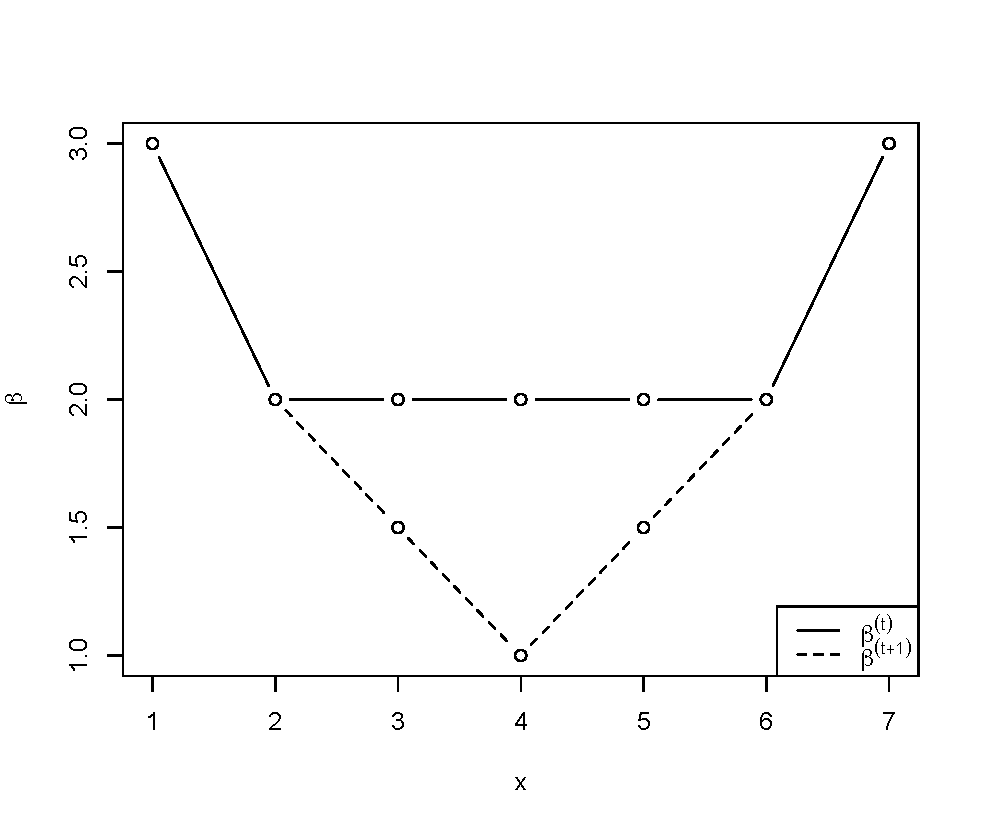
\includegraphics[width = 8cm]{ActivePoint2.pdf}}
	\caption[Active Set Parameterization: Inverse Convex]{$\beta_4^{*(t+1)} = \beta_4^{*(t) }-1$}
	\end{figure}		
	
 Because of the inverse convex constraints, it is natural to consider the KKT conditions (Kuhn and Tucker 1951) which are necessary for an estimate to be a local maximum. Let us define
	
	\[
	\text{KKT error} = {\text{max}} 
	\begin{cases}
		|\frac{\partial \ell } {\partial \beta_i^*}|, & \text{if } \Delta_{i-1} < \Delta_{i} + \xi \\
		\text{max}_i(\frac{\partial \ell}{\partial \beta_i^*},0 ) , & \text{if } \Delta_{i-1} \geq \Delta_i + \xi \\  
	\end{cases}
	\]
	
	We define the inverse convex estimator as having KKT error of 0 for all points. In addition, if $i$ is an active point, then we further require that $\frac{\partial \ell^2 } {\partial (\beta_i^*)^2} \leq 0$. In our implementation, we consider the solution to have been achieved if the KKT error was less than $10^{-4}$. 
	
	It is not clear that the inverse convex estimator is unique. In the case of the Gaussian mixture, it is well known that there can be multiple distinct modes with finite likelihood and that different initial values often lead to different solutions. To test if the inverse convex estimator is unique, we simulated 50 sampled data points from a standard normal distribution and ran the algorithm presented in the next section from a uniform initial estimate, a initial estimate which concentrated mass toward the left side and finally a initial estimate which concentrated mass toward the right side. We recorded the maximum difference of estimated density at each of the data points in the data set. This was repeated 1,000 times. Over all 1,000 simulated datasets, the maximum difference in estimated density was $4.4 \times 10^{-5}$, suggesting that multiple modes is not likely to be an issue for this estimator. 
	
{\section{Algorithm} }
	
	In this chapter, we will only briefly describe the algorithm, as it is a simplified version of the algorithm found in Anderson-Bergman and Yu 2014 and Anderson-Bergman 2014. 
	
	 The nature of the problem is very similar to finding the log-concave estimator. The has been done efficiently with the Active Set Algorithm (ASA), presented in D\"umbgen \emph{et al.} (2011). The ASA procedure starts with a minimal set of active points and maximizes over this set, adding new active points and optimizing until the algorithm has converged. Constrained optimization over these sets is done via Sequential Quadratic Programming (SQP). This is a very efficient algorithm, as the number of active points in the solution tends to be considerably smaller than the total number of knots considered ($n$). 
	
	A further complication of the inverse convex estimator compared with the log-concave NPMLE without censoring is that the inverse convex likelihood function is not guaranteed to be concave. SQP will fail if the function is not locally concave at any step of the algorithm. A similar problem was faced when finding the log-concave NPMLE for interval censored data in chapter 3. We will use the same technique to address this problem. To insure convergence of the algorithm, we included a univariate optimization step. This step would optimize the active set parameters one at a time and could increase the likelihood function even when not locally concave via the bisection method. While this insured convergence, it was too slow to be used by itself, so our algorithm contained both an SQP step and a univariate optimization step. Typically, the likelihood function was not locally concave in only the first step or two of the algorithm, so rather than modifying the SQP step as we did in chapter 3, we merely skipped the SQP step if the likelihood function was found to be locally non-concave. 

	Two further modifications were required to deal with the inverse convex problem. The first issue was that while that while the likelihood function was defined for all real values of the parameters in the log-concave case, the likelihood function for the inverse convex estimator is undefined if $\beta_i \leq 0$. This was dealt with by half-stepping if the proposed steps were beyond the boundary. The second issue is that we would like the algorithm to terminate if we are convinced that it has entered a domain of attraction to a degenerate distribution. To do this, we terminated the algorithm and returned an error report if the estimated density, normalized by the empirical standard deviation of the dataset, was ever greater than a pre-specified $d_{max}$. In our implementation, we set $d_{max} = 10^7$. 
	
	To test how often the algorithm would terminate early due to approaching a degenerate mode, we sampled data from an $F_{1,1}$ and an $F_{1,2}$ distribution. The $F_{1,1}$ was chosen because the unbounded density suggests it would behave worse than the $F_{1,2}$, which has bounded density but very heavy tails. The $F_{1,1}$ distribution is not inverse convex while the $F_{1,2}$ is on the boundary of inverse convex as mentioned in section 2. We tested data with samples sizes $n$ = 10, 15, 20 and 25. For each $n$, we creating $MC = 1,000$ samples. We found that the estimated probability of terminating due to approaching a degenerate mode for each sample size was 0.353, 0.107, 0.003 and 0 respectively for the $F_{1,1}$ distribution and 0.302, 0.014, 0 and 0 for the $F_{1,2}$. In addition, the algorithm never terminated due to approaching a degenerate mode in our simulations in the next section. This suggests that while the unbounded likelihood is a theoretic issue with the inverse convex estimator, in practice our algorithm finds the local mode of interest reliably for datasets with $n \geq 25$. 
	
	We found this algorithm to be sufficiently fast for investigating the properties of the estimator for moderate sized data sets. For $n$ = 1,000, the algorithm typically converged in under 2 seconds (2007 Macbook with 2 GHz Intel Core 2 Duo processor, 4 GB of RAM). However, we ran into problems with larger datasets. In sample sizes of $n$ = 10,000,  we occasionally ran into numeric problems regarding the constraints in the quadratic programming routine. When the algorithm did converge, it typically took around 1 minute. We do note that our algorithm converged on all of the datasets we used in our real data applications in section 6, including 4 datasets of approximately $n = 7,000$ and one data set of $n = 28,155$. For the largest dataset, the algorithm converged in just under 5 minutes. We still caution that simulated data suggests that the algorithm will not generally be reliable for datasets of that size in its current implementation. Further work is necessary to develop a reliable algorithm for large datasets.
	
{\section{Simulations} } 

	One of the motivations for shape constrained inference is density estimation. Our motivation for investigating the inverse convex estimator began with estimating survival curves for interval censored data. Because of this, we will use simulations to compare both density estimation and survival estimation for the log-concave NPMLE and the inverse convex estimator. 
	
	We compared five different distributions. These were a standard normal, a gamma(2,2), a t-distribution with 3 degrees of freedom, an F-distribution with $\nu_1 = 3, \nu_2 = 3$ and a gamma(0.5, 0.5). Note that the normal and gamma(2,2) distribution are both log-concave but the remaining distributions are not. All of the distributions are inverse convex with the exception of the gamma(0.5, 0.5) which has unbounded density at 0. For each of these distributions, we will examine the estimated density at the true median, the estimated median and the estimated $90^{th}$ percentile. We consider sample sizes of $n$ = 50, 100 and 500. For each sample size, we will generate $MC = 1,000$ simulated datasets and fit each estimator to each dataset.  The means and standard deviations for the various estimates can be seen on tables 2 - 4 in the appendix. We also provide sample plots of the estimated density and cumulative distributions function for the t and F distributions with $n = 1,000$ in figure 3. 
	
	\begin{figure}[H]
	\centerline{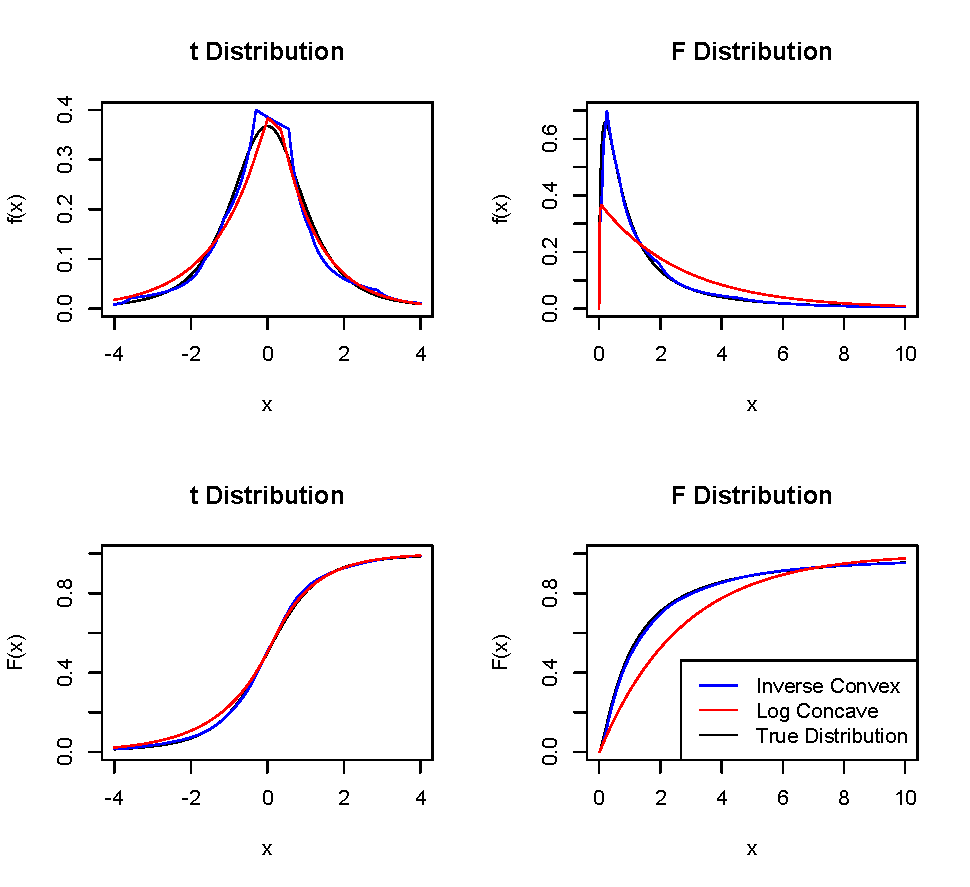
\includegraphics[width = 11cm]{SamplePlots.pdf} }
	\caption[Inverse Convex and Log-concave Estimators for Simulated Data]{Inverse convex and log-concave estimators based on random sample of $n= 500$ from a $t_3$ and $F_{3,3}$ distribution }
	\end{figure} 

	
	In our simulations, we saw a few trends. For log-concave distributions, the log-concave estimator had lower standard deviations for all estimators, although the magnitude of this advantage varied. For density estimation, the reduction was significant, but for survival estimation the reduction was marginal. In addition, as $n$ increased, the relative advantage decreased. At $n = 500$ for log-concave simulated data, the estimators were nearly equivalent. We noticed that the log-concave estimator does a surprisingly good job of estimating the non log-concave t-distribution. We speculate that there are two reasons for this. First is that the t-distribution is only mildly non log-concave. In fact, the t-distribution is log-concave on the interval $[-\sqrt{\nu}, \sqrt{\nu}]$, where $\nu$ = degrees of freedom. Secondly, the t-distribution is symmetric. This means the log-concave constraint ``pulls" evenly from both sides of the mode. In contrast, we see the log-concave estimator suffers extreme bias when estimating the F and gamma(0.5, 0.5) distributions. The inverse convex estimator handles these distributions very well. Finally, we found that the inverse convex estimator did suffer from bias when estimating the gamma(0.5,0.5) distribution. However, these biases were very minor compared with biases the those that the log-concave estimator displayed. These simulations suggest that the inverse convex estimator would be preferred if the there were concerns of heavy tails, especially if the data were skewed.  

	
		
{\section{Real Data Application} }
	
	The characteristics of the inverse convex estimator can be summarized as unimodal, allowing for skew and very heavy tails. There are many areas of research for which this describes the type of data to be expected. As an illustrative example, we will examine a few wage and income data sets. Moscarini (2005) describes an ideal wages model to have a unique interior mode, skewness and a long and fat right tail. Income may be further right skewed than wages, as it includes investments as well. This is the type of data we expect the inverse convex estimator to do quite well with. 
	
	We first considered a dataset collected by the Philippines' National Statistics Office. This dataset can be found in the publicly available CRAN package ``ineq", titled ``Ilocos". The dataset contains 632 subjects and their reported income, along with other covariates. One individual reported 0 income. We dropped this individual from our dataset for two reasons. First, typical parametric models for income, such as log normal, do not allow for 0 income. It should be noted that the log-concave and inverse convex models would not have such problems. However, it is more reasonable to model income as a mixture of those with no reported income and those with positive reported income. Therefore we will only model the income of individuals with positive reported income. Of these individuals, 116 came from the province La Union and 381 were from Pangasinan. 
	
	We would like to examine the fits of various models to the distribution of wealth in the two provinces. We will do this by comparing estimated probability densities and cumulative distribution functions with histograms and the empirical distribution functions. In addition, we will examine the Lorenz Curve and Gini coefficient, classic econometrics measures of disparity within a society. The Lorenz Curve states $x$ proportion of the poorest subjects in a society own $y$ proportion of the wealth (or in this case, income). The Gini coefficient is equal to $1 - 2 \displaystyle \int_0^1 L(x) \mathrm{d}x$, where $L(x)$ is the Lorenz curve, or a one number summary of the Lorenz curve. The Gini coefficient ranges from 0 to 1 (assuming only non negative measures of wealth), with 0 being perfectly evenly distributed wealth in the society and $\frac{N-1} {N}$ if 100\% of the wealth belongs to only one individual. Larger values of the Gini coefficient corresponds with more disparity within a society. 	The estimated Lorenz curve and Gini coefficient can be  calculated from an estimated cumulative distribution function. 

	We  fit three models and compared the fits of each model. For shape constrained models, we  fit the inverse convex and log-concave models. We also fit a log normal model, as this is a classic parametric model used for income. We used the Empirical Distribution Function to check the fits of our model. The fits can be seen on figure 2. We only plotted the fits up until 300,000 pesos/year to make the plots easier to examine. 
	
	\begin{figure}
	\centerline{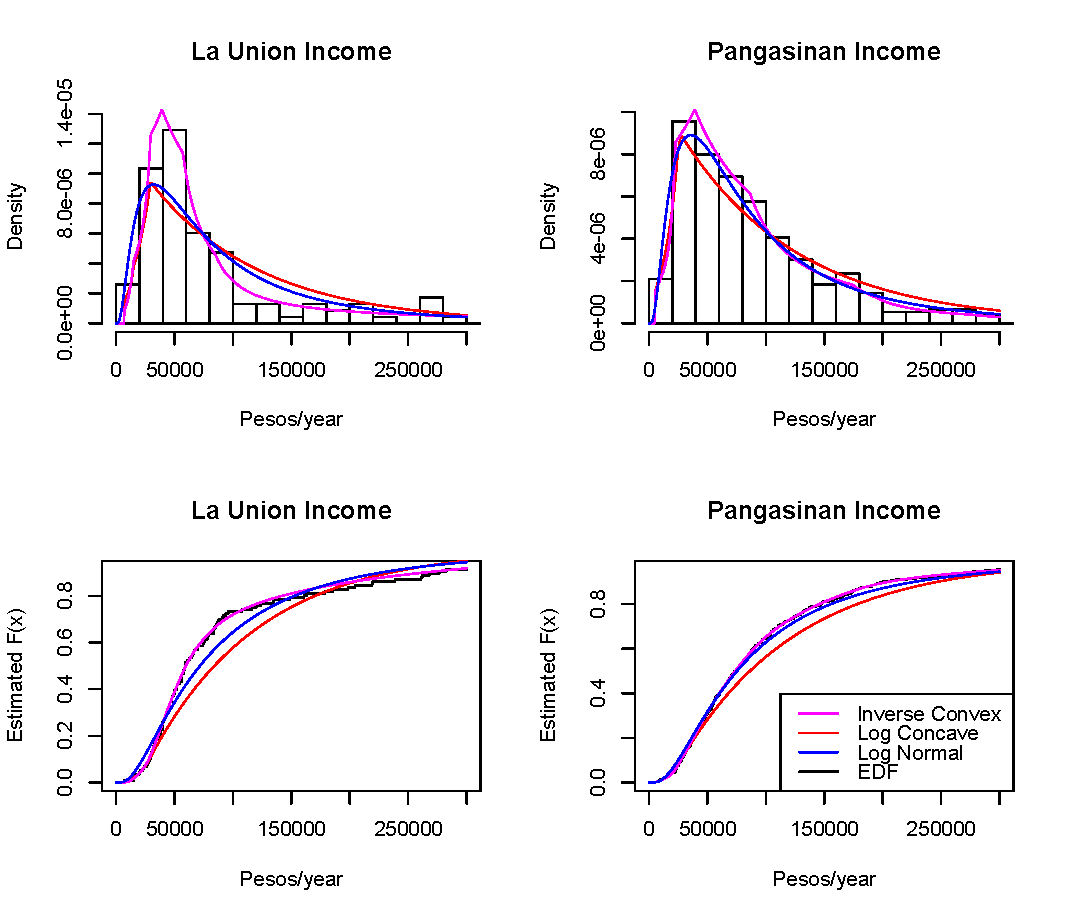
\includegraphics[width = 14cm]{MEDens.pdf} }
	\caption{Fits of the Distribution of Income in the Pangasinan and La Union Provinces}
	\end{figure} 	
	
	Examining the fits, the inverse convex estimator matches the empirical distribution function much better than the log-concave estimator, while still providing a smooth estimated cdf and valid density estimates (the EDF does not). The log normal estimator fits the EDF considerable better than the log-concave estimator, but still not as well as the inverse convex estimator. The log-concave estimator is unable to properly model the heavy tails of the distribution. Although the overall fit of the inverse convex estimator is very good, we do note that there is some disagreement around 20,000 pesos/year in the La Union cdf between the inverse convex and EDF estimates. Given the smaller sample size of the La Union ($n$ = 116), we believe the observed difference between the EDF and inverse convex fit is just noise rather than systematic mis-modeling. Despite this, the inverse convex still looks to be a much better fit than the other models for the La Union data. In the Pangasinan data, the inverse convex estimates look to be an unquestionably good fit. 


	\begin{figure}
	\centerline{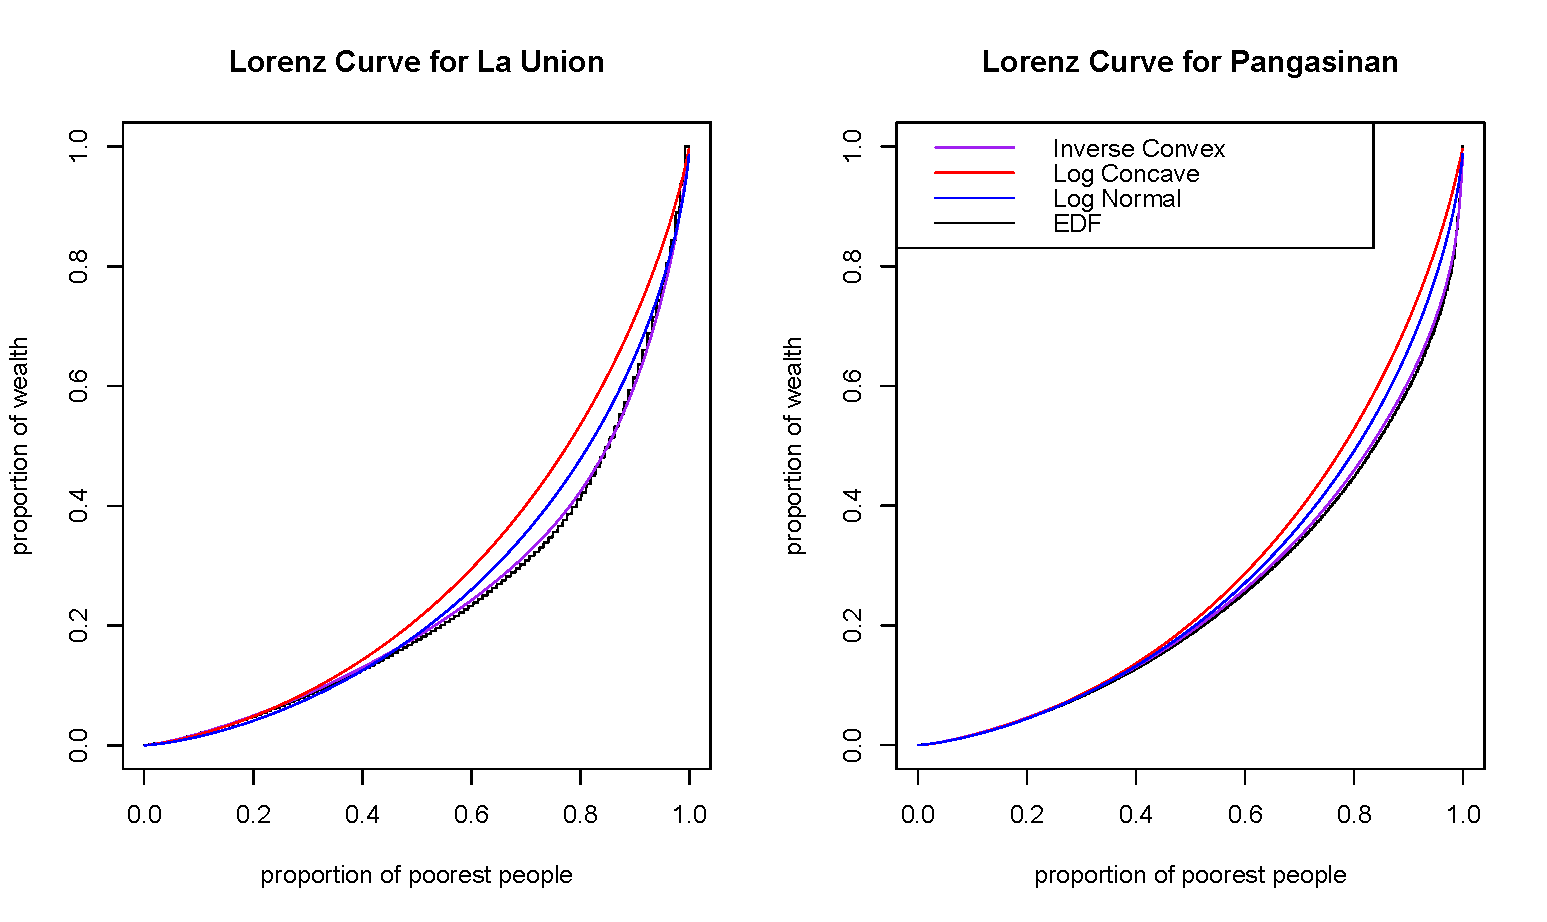
\includegraphics[width = 14cm]{LCurves.pdf} }
	\caption{Lorenz Curves for the Pangasinan and La Union Provinces}
	\end{figure} 	
	
	We see a similar trend in the Lorenz curves. The inverse convex estimator appears to be a smoothed version of the EDF. We can see a strong systemic difference between the log normal and the EDF curves. The bias appears even higher for the log-concave curve. 		
	Finally, for each model we computed the Gini coefficient for both populations and created a 95\% bootstrap CI using $B = 1,000$ bootstrap samples. These are presented on table 1. We note that the inverse convex estimates agree the most with the empirical estimate and we suspect that the greater observed differences for the log-concave and log normal models is due in part with these models not allowing for heavy enough tails. While the difference in Gini coefficients was not statistically significant in any of the groups, we note that the log-concave estimate reversed the ranking of the estimates compared to the other estimators. We were surprised that the empirical bootstrap confidence intervals for the La Union group ($n = 116$) were narrower than the inverse convex confidence intervals. A literature review on the topic revealed that bootstrap confidence intervals for the Gini coefficient typically are too narrow for smaller samples (Dixon \emph{et al.} 1987), so we believe this is responsible for the narrower confidence interval based on the empirical estimator. 
	
	\begin{table}

\begin{center}	
\caption[Estimated Gini Coefficients from Different Model Fits]{Estimated Gini coefficients for each model. Values in parentheses are bootstrapped 95\% CIs}

\begin{tabular} {| c | c | c |} 

	
	\hline
	Model			&	La Union			&	Pangasinan 	\\
	\hline
	
	Empirical			&	0.514 (0.459, 0.569)			&	0.502 (0.436, 0.568)		\\
	\hline
	
	Inverse Convex	&	 0.500 (0.440, 0.560)		&	0.488 (0.427, 0.549)		\\
	\hline
	
	log-concave		&	0.422 (0.426, 0.490)			&	0.433 (0.410, 0.456)		\\
	\hline
	
	Log Normal		&	0.474  (0.420, 0.528)		&	0.458 (0.420, 0.496)		\\
	
	 \hline
	 
\end{tabular}

\end{center}	 

\end{table}

	In this example, the inverse convex estimator appeared to fit the data very well, with the log normal providing a slightly worse fit but still much better than the log-concave fit. This was not always the case. We examined several income and wage data sets and while the inverse convex fit always appeared to be the best fit, in some datasets the log-concave fit appeared a superior fit compared to the log normal. The general trend we found was that datasets with more disparity (\emph{i.e.}\ higher Gini coefficients) tended to be better fit by the log normal distribution, while datasets with less disparity tended to be better fit by the log-concave fit. This trend would be expected, as the log-concave fit should be more flexible than log normal in general, but will break down for heavy tailed data. We emphasize again that in both situations, the inverse convex estimator appeared to be the best fit of the three considered. 
	
	 To demonstrate this general trend we found, we present the data set ``CPS1988", found in the CRAN package ``AER". This dataset contains wage data collected from the March 1988 Current Population Survey conducted by the US Census Bureau. A total of 28,155 subjects are included in the dataset. They are divided into 4 different regions, Northeast ($n = 6,441$), Midwest ($n = 6,863$), South ($n = 8,760$) and West ($n = 6,091$). Wages are given in weekly salaries. We plotted the fitted cdf's for each region individually and also all regions aggregated using the same models as before. Again, we zoom into the interval (500, 2,000) to allow easier comparison of fits (maximum observed value was 18,777). We also list the Gini coefficient, as calculated by the empirical distribution model. Fits are presented on figure 6 and figure 7. 

	\begin{figure}[H]
	\centerline{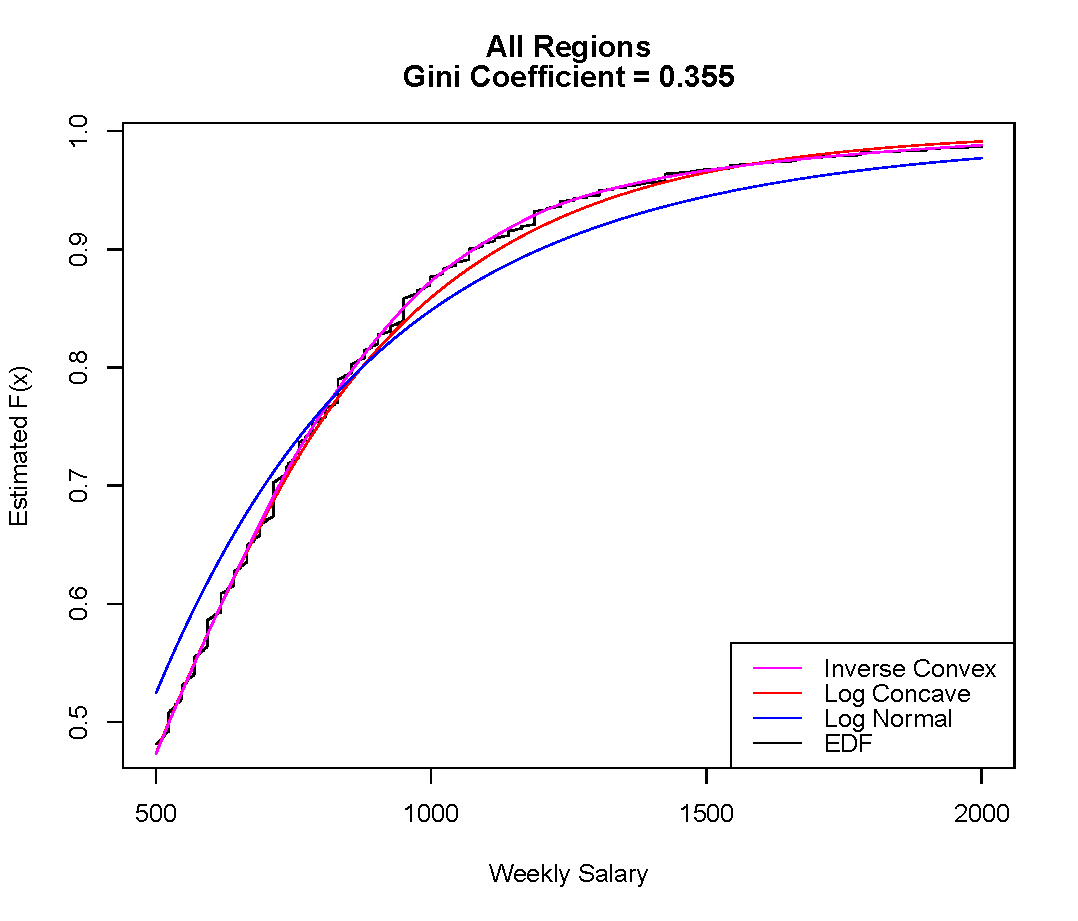
\includegraphics[width = 14cm]{CombineRegions.pdf} }
	\caption{Estimated wage cdf from CPS1988 dataset}
	\end{figure} 	
	

	\begin{figure}[H]
	\centerline{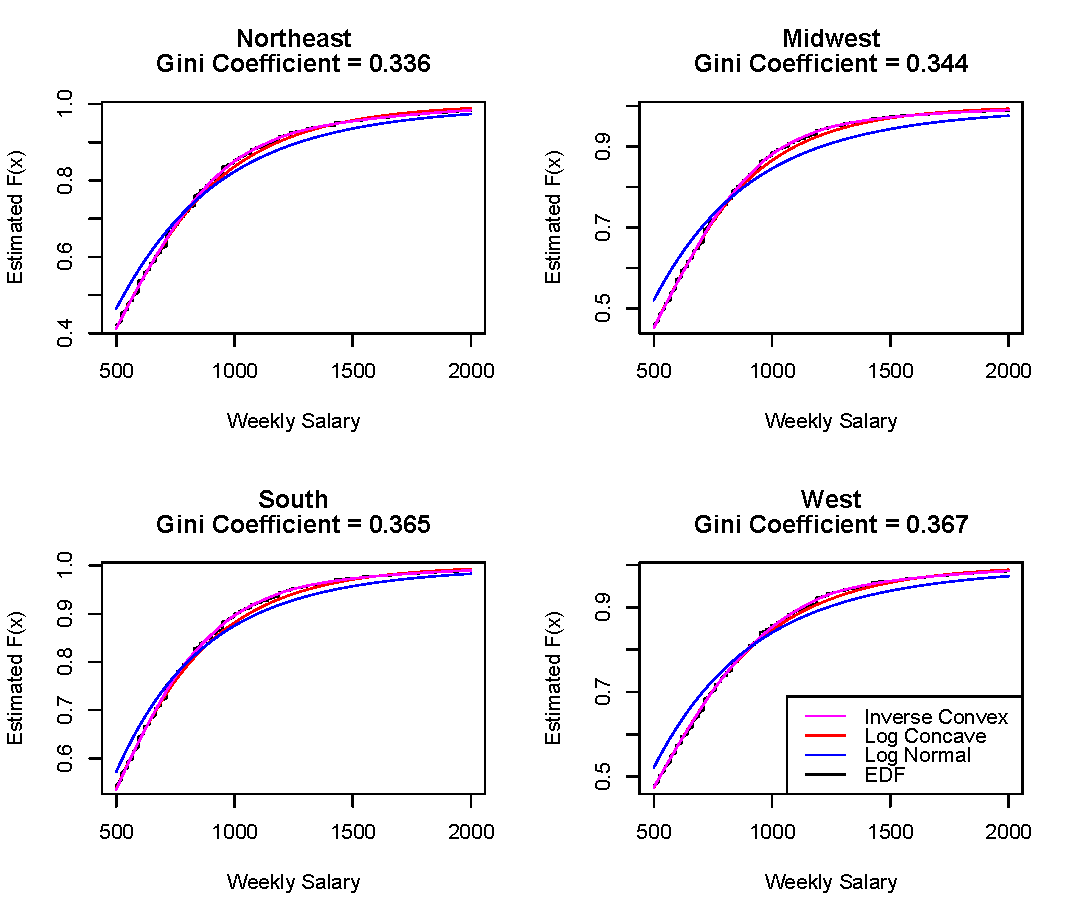
\includegraphics[width = 14cm]{IndividualRegions.pdf} }
	\caption{Estimated wage cdf's by region from CPS1988 dataset}
	\end{figure} 	
	
	We note that in this case, the inverse convex again appears to be the best fit in all scenarios. However, this time the log-concave does fairly well and the log normal does  poorly. The fact that the inverse convex estimator always appears to fit best and both of the other estimators can suffer heavy bias under different scenarios makes the inverse convex estimator a very attractive choice. 
	
{\section{Conclusion} }

	The inverse convex constraint leads to a very flexible unimodal shape constraint, allowing for very heavy tails but not allowing for unbounded density. Theory dictates that the family of inverse convex functions is more flexible than the log-concave family, as the log-concave family is properly contained within the inverse convex family. The inverse convex estimator does have the theoretic problem of an unbounded likelihood function leading to a degenerate maximum likelihood estimate. However, in practice it is quite easy to avoid these degenerate estimates and find a more useful local maximum as an estimate. Simulations show us that the inverse convex estimator is nearly as efficient as the log-concave estimator for quantile estimation when the true distribution is log-concave, although the log-concave estimator may be preferred for density estimation for smaller samples. We found the log-concave estimator suffered from heavy bias from heavy right skewed distributions. The inverse convex estimator behaved very well when estimating quantiles of unimodal heavy tailed distributions, even when the inverse convex assumptions was violated due to unbounded density. Applying the estimator to real data, we see that the inverse convex estimator can fit income and wage data much better than the log-concave or log normal distribution, both of which suffered heavy bias under different scenarios. We would recommend the inverse convex for modeling of distributions in which the investigator may be concerned with skewed heavy tails. 
	
	We are particularly interested in applying the inverse convex estimator to censored data, although currently an algorithm for such data has not been implemented. Another proposed research topic on the inverse convex estimator would be to find formal bounds on the domain of attraction toward the degenerate estimate. We are interested in finding a function such that when $f(\beta,x) < \xi$, $\beta$ was insured to be outside the domain of attraction. This would both help our algorithm in smaller samples and help define the limitations of the inverse convex estimator. 


{\section{Appendix}}

Anderson-Bergman, C., (2014) Semi and Non-Parametric Methods for Interval Censored Data with Shape Constraints, PhD Dissertation, University of California Irvine

\vspace{3mm}

Anderson-Bergman, C. and Yu,Y.,  (2014) Computing the Log Concave NPMLE for Interval Censored Data, \emph{preprint}

\vspace{3mm}


Chang, G., Walther, G. (2007), Clustering with Mixtures of Log-Concave Distributions, \emph{Computational Statistics and Data Analysis}, Vol 51, No. 12, 6242-6251

\vspace{3mm}

Dixon, P., Weiner, J., Mitchell-Olds, T., Woodly, R. (1987), Bootstrapping the Gini Coefficient of Inequality, \emph{Ecology}, Vol 68, 1548-1551

\vspace{3mm}

D\"umbgen, L., H\"usler, A., Rufibach, K. (2011), Maximum Likelihood Estimation of a Log-Concave Density Based on Censored Data, preprint

\vspace{3mm}

D\"umbgen, L., Rufibach, K. (2009), Maximum Likelihood Estimation of a Log-Concave Density and its Distribution Function: Basic Properties and Uniform Consistency, \emph{Bernoulli}, Vol 15 No. 1 40-68

\vspace{3mm}

Grenander, U. (1956), On the Theory of Mortality Measurement. Part II, \emph{Scandinavian Actuarial Journal} Vol 39, 125-131

\vspace{3mm}

Groeneboom, P. (1991), Nonparametric Maximum Likelihood Estimation for Interval Censored Data, \emph{Technical Report}, Statistics Department, Stanford University

\vspace{3mm}

Kuhn, W., Tucker, W. (1951), Nonlinear Programming, \emph{Proceedings of 2nd Berkeley Symposium}, 481-492

\vspace{3mm}

Moscarini, G., (2005), Job Matching and the Wage Distribution, \emph{Econometrica}, Vol 73, No. 2 481-516

\vspace{3mm}

Rufibach, K. (2007), Computing Maximum Likelihood Estimators of a Concave Density, \emph{Journal of Statistical Computation and Simulation}, Vol 77, No. 7, 561-574

\vspace{3mm}

Wegman, E. (1969), A Note on Estimating a Unimodal Density, \emph{The Annals of Mathematical Statistics}, Vol 40 No. 5, 1661-1667

\vspace{3mm}



{\section{Appendix}	}


		\begin{table}

\begin{center}	
\caption[Simulated Comparisons for Inverse Convex and Log-concave Estimators with $n = 50$]{Simulated Comparisons with $n = 50$ based MC = 1000 simulations. Values in parentheses are standard deviations. ``Density" refers to estimated density at the true median. $90^{th}$ Perc refers to the $90^{th}$ percentile.}

\begin{tabular} {| c | c | c | c | c | c | c |} 


	 \hline
	 
	 n = 50 		& 			&	True Values	& Inverse Convex		&	log-concave	\\
	 
	 \hline
	 
	N(0,1) 		& Density		& 	0.40			& 	0.42 (.090)		&	0.40 (.065)	\\
	 
	 
		 		& Median 		&	0			& 	0.00 (.166)		&	0.00 (.158)	  \\ 
					
				& $90^{th}$ Perc&	1.28			& 	1.22 (.222)		&	1.27 (.214)	\\
	
	\hline

	 
	 Gamma	 	& Density		& 	0.63			& 	0.65 (.132)		&	0.62 (.084)	\\
	 
	 
	 (2,2)			& Median 		&	0.84			& 	0.83 (.104)		& 	0.86 (.097)	 \\ 
				
				& $90^{th}$ Perc&	1.94			& 	1.89 (.234)		&	1.94 (.221)	 \\
	
	\hline
		
	 
	 $t_3$	 	& Density		& 	0.37			& 	0.38 (.098)		&	0.34 (.061)	\\
	 
	 
	 			& Median 		&	0			& 	0.00 (.186)		& 	0.00 (.182)	  \\ 
				
				& $90^{th}$ Perc&	1.64			& 	1.55 (.366)		&	1.76 (.411)	 \\
	
	\hline
	
		 
	 $F_{3,3}$	 	& Density		& 	0.32			&  0.33 (.073)			&	0.27 (.063)	\\
	 
	 
	 			& Median 		&	1			& 0.97 (.202)			& 	2.00 (1.33)	  \\ 
				
				& $90^{th}$ Perc&	5.39			& 5.21(1.68)	 		&	6.50 (4.42)	 \\
	

	\hline
	
		 
	 Gamma		& Density		& 	0.47			& 0.45 (.082)			&	0.64 (.066)	\\
	 
	 
	 (0.5,0.5)		& Median 		&	0.45			& 0.35 (.122)			& 	0.70 (.138)	  \\ 
				
				& $90^{th}$ Perc&	2.71			& 2.53 (.542)			&	2.29 (.449)	 \\
	


	\hline		
	
\end{tabular}
\end{center}

\end{table}
	
	

\begin{table}

{

\begin{center}	
\caption[Simulated Comparisons for Inverse Convex and Log-concave Estimators with $n = 100$]{Simulated Comparisons with $n = 100$ based MC = 1000 simulations. Values in parentheses are standard deviations. ``Density" refers to estimated density at the true median. $90^{th}$ Perc refers to the $90^{th}$ percentile.}

\begin{tabular} {| c | c | c | c | c | c | c |} 


	 \hline
	 
	 n = 100 		& 			&	True Values	& Inverse Convex		&	log-concave	\\
	 
	 \hline
	 
	N(0,1) 		& Density		& 	0.40			& 	0.41 (.066)		&	0.40 (.053)	\\
	 
	 
		 		& Median 		&	0			& 	0.00 (.115)		&	0.00 (.112)	  \\ 
					
				& $90^{th}$ Perc&	1.28			& 	1.24 (.150)		&	1.28 (.145)	\\
	
	\hline

	 
	 Gamma	 	& Density		& 	0.63			& 	0.65 (.096)		&	0.62 (.065)	\\
	 
	 
	 (2,2)			& Median 		&	0.84			& 	0.84 (.076)		& 	0.85 (.072)	 \\ 
				
				& $90^{th}$ Perc&	1.94			& 	1.90 (.170)		&	1.95 (.160)	 \\
	
	\hline
		
	 
	 $t_3$	 	& Density		& 	0.37			& 	0.37 (.062)		&	0.35 (.046)	\\
	 
	 
	 			& Median 		&	0			& 	0.00 (.124)		& 	0.00 (.124)	  \\ 
				
				& $90^{th}$ Perc&	1.64			& 	1.59 (.256)		&	1.77 (.309)	 \\
	
	\hline
	
		 
	 $F_{3,3}$	 	& Density		& 	0.32			&  	0.33 (.052)		&	0.26 (.052)	\\
	 
	 
	 			& Median 		&	1			& 	0.99 (.144)		& 	0.70 (1.01)	 \\ 
				
				& $90^{th}$ Perc&	5.39			& 	5.31 (1.24)		&	6.67 (3.34)	 \\
	

	\hline
	
		 
	 Gamma		& Density		& 	0.47			& 0.44 (.054)			&	0.63 (.048)	\\
	 
	 
	 (0.5,0.5)		& Median 		&	0.45			& 0.36 (.090)			& 	0.70 (.099)	  \\ 
				
				& $90^{th}$ Perc&	2.71			& 2.63 (.438)			&	2.31 (.326)	 \\
	


	\hline		
	
\end{tabular}
\end{center}
}

\end{table}


\begin{table}

\begin{center}	
\caption[Simulated Comparisons for Inverse Convex and Log-concave Estimators with $n = 500$]{Simulated Comparisons with $n = 500$ based MC = 1000 simulations. Values in parentheses are standard deviations. ``Density" refers to estimated density at the true median. $90^{th}$ Perc refers to the $90^{th}$ percentile.}

\begin{tabular} {| c | c | c | c | c | c | c |} 


	 \hline
	 
	 n = 500 		& 			&	True Values	& Inverse Convex		&	Log-concave	\\
	 
	 \hline
	 
	N(0,1) 		& Density		& 	0.40			& 	0.40 (.032)		&	0.40 (.030)	\\
	 
	 
		 		& Median 		&	0			& 	0.00 (.055)		&	0.00 (.054)	  \\ 
					
				& $90^{th}$ Perc&	1.28			& 	1.27 (.070)		&	1.28 (.069)	\\
	
	\hline

	 
	 Gamma	 	& Density		& 	0.63			& 	0.63 (.049)		&	0.63 (.039)	\\
	 
	 
	 (2,2)			& Median 		&	0.84			& 	0.84 (.036)		& 	0.84 (.035)	 \\ 
				
				& $90^{th}$ Perc&	1.94			& 	1.93 (.077)		&	1.95 (.071)	 \\
	
	\hline
		
	 
	 $t_3$	 	& Density		& 	0.37			& 	0.37 (.034)		&	0.37 (.030)	\\
	 
	 
	 			& Median 		&	0			& 	0.00 (.057)		& 	0.00 (.057)	  \\ 
				
				& $90^{th}$ Perc&	1.64			& 	1.62 (.122)		&	1.75 (.151)	 \\
	
	\hline
	
		 
	 $F_{3,3}$	 	& Density		& 	0.32			&  	0.33 (.052)		&	0.26 (.052)	\\
	 
	 
	 			& Median 		&	1			& 	0.99 (.144)		& 	0.70 (1.01)	 \\ 
				
				& $90^{th}$ Perc&	5.39			& 	5.31 (1.24)		&	6.67 (3.34)	 \\
	

	\hline
	
		 
	 Gamma		& Density		& 	0.47			& 0.43 (.036)			&	0.64 (.022)	\\
	 
	 
	 (0.5,0.5)		& Median 		&	0.45			& 0.36 (.051)			& 	0.69 (.044)	  \\ 
				
				& $90^{th}$ Perc&	2.71			& 2.75 (.494)			&	2.30 (.146)	 \\
	


	\hline		
	
\end{tabular}
\end{center}

\end{table}

 
 \end{document}
	